%%%%%%%%%%%%%%%%%%%%%%%%%%%%%%%%%%%%%%%%%%%%%%%%%%%%%%%%%%%%%%%%%%%%%%%
%% Vorlage f�r Abschlussarbeiten                                     %%
%%-------------------------------------------------------------------%%
%% Datei:        methods.tex                                         %%
%% Beschreibung: Methodenteil, der beschreibt welche Hard- oder      %%
%%               Software bereits vorhanden ist.                     %%
%%               und ein Ausblick KURZ auf ca einer bis max zwei     %%
%%               Seiten zusammengefasst.                             %%
%% Autor: 			 Stefan Herrmann                                     %%
%% Datum:        28.11.2012                                          %%
%% Version:      1.1.0                                               %%
%%%%%%%%%%%%%%%%%%%%%%%%%%%%%%%%%%%%%%%%%%%%%%%%%%%%%%%%%%%%%%%%%%%%%%%

\chapter{Methoden}
\index{Methoden} %% Eintrag im Stichwortverzeichnis
In wissenschaftlichen Arbeiten wird in diesem Kapitel aufgef�hrt, was untersucht wurde. Dazu geh�rt die Beschreibung von eingesetzten Algorithmen, Programmen und Versuchsaufbauten. Generell ist f�r uns hier im Institut 4 wichtig, dass man zwischen vorhandener Soft- bzw. Hardware und ihrer eigenen Leistung unterscheiden kann. Insofern wird hier die Festlegung getroffen, dass in den Methodenteil nur diejenigen Abschnitte kommen, die vorhandene Hard- und Software beschreiben. Dar�ber hinaus k�nnen hier Versuchsaufbauten beschrieben werden.

\section{Software}
In diesem Kapitel wird Software beschrieben, welche f�r die Erf�llung der gestellten Aufgabe verwendet wurde: Also solche Anwendungen, die nicht selber geschrieben wurden. Hierzu z�hlen auch Programme, die von anderen Studenten in Abschlussarbeiten programmiert wurden. Es geht dabei darum, einen kurzen �berblick zu gew�hren. Es soll nicht jedes Fenster als Screenshot eingebunden werden. Wird beispielsweise die Anwendung Keil hier aufgef�hrt, so reicht ein kurzer Absatz mit Quellenverweis auf die Webseite. Wichtig in diesem Absatz ist nicht unbedingt, wie dieses Programm bedient wird, sondern vielmehr welche Version eingesetzt wurde, ob Zusatzmodule ben�tigt werden oder ob gewisse Funktionen deaktiviert werden m�ssen.

Im Rahmen dieser Vorlage werden jetzt zwei Programme und deren Installation erl�utert, weil diese f�r das Erstellen einer schriftlichen Ausarbeitung ben�tigt werden. Hierbei handelt es sich um eine Umgebung f�r das Latex Textsatzsystem, was die Bearbeitung dieser Vorlage erm�glicht.

\subsection{Miktex}
\index{Miktex}
Bei MiKTeX handelt es sich um eine TeX-Distribution f�r Windows. Es wird empfohlen, diese komplett zu installieren. Die neuesten Installationsdateien sind im Internet unter \textit{http://miktex.org/download} zu finden. Hier sollte der MiKTeX Net Installer heruntergeladen und ausgef�hrt werden. Nach dem Ausf�hren m�ssen zun�chst die notwendigen Dateien heruntergeladen werden, vergleiche Abbildung \ref{fig:Miktex02} und \ref{fig:Miktex03}.

\begin{figure}
	\centering
		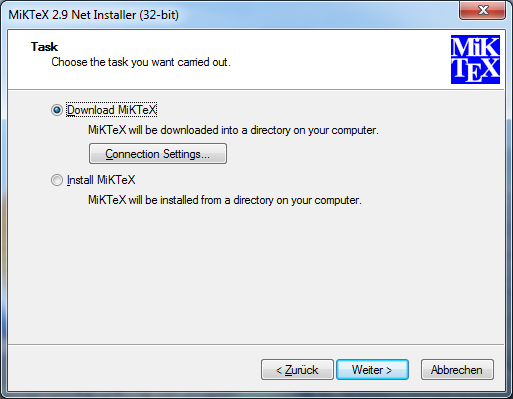
\includegraphics[width=0.60\textwidth]{images/methods/Miktex02.png}
	\caption{Herunterladen der MiKTeX Dateien.}
	\label{fig:Miktex02}
\end{figure}
 
\begin{figure}
	\centering
		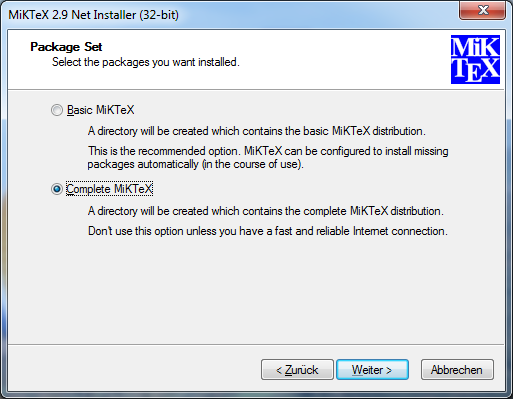
\includegraphics[width=0.60\textwidth]{images/methods/Miktex03.png}
	\caption{Ausw�hlen der kompletten Distribution.}
	\label{fig:Miktex03}
\end{figure} 

Nach dem Abschluss des Download Programmes muss die Installationsroutine aus dem Download Ordner gestartet werden. Im Zuge der Installation ist auszuw�hlen, dass die komplette Distribution installiert werden soll und dass die bevorzugte Blattgr��e A4 ist, vergleiche Abbildung \ref{fig:Miktex09} und \ref{fig:Miktex12}.

\begin{figure}
	\centering
		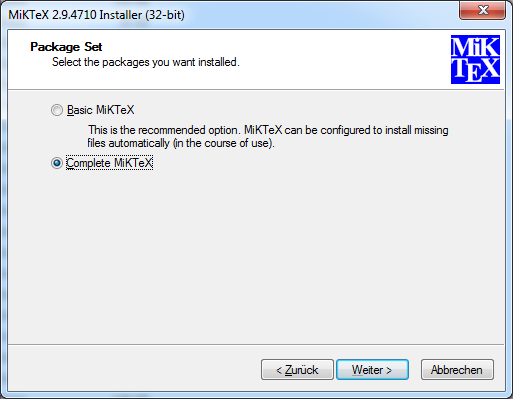
\includegraphics[width=0.60\textwidth]{images/methods/Miktex09.png}
	\caption{Installation der kompletten Distribution.}
	\label{fig:Miktex09}
\end{figure}
 
\begin{figure}
	\centering
		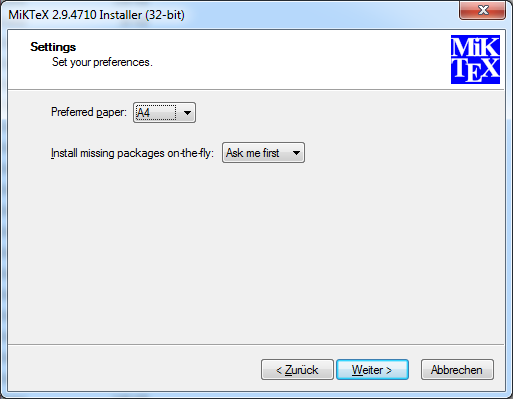
\includegraphics[width=0.60\textwidth]{images/methods/Miktex12.png}
	\caption{Bevorzugte Papiergr��e einstellen.}
	\label{fig:Miktex12}
\end{figure} 



\subsection{TexnicCenter}
\index{TexnicCenter}
Bei TexnicCenter handelt es sich um einen Editor, um Latex-Dokumente zu erstellen. Dieser sollte erst nach der Installation von MiKTeX eingerichtet werden. Hierbei sollte die "`Typische"' Installation gew�hlt werden, Abbildung \ref{fig:Texniccenter03}.


\begin{figure}
	\centering
		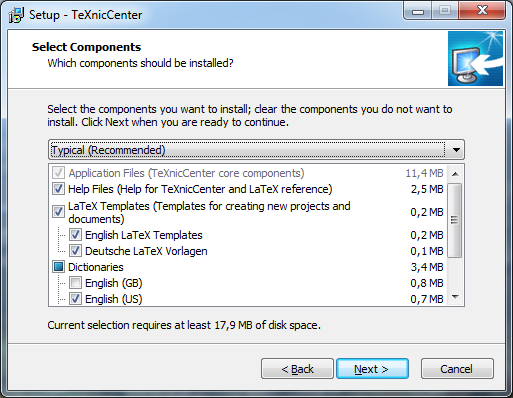
\includegraphics[width=0.60\textwidth]{images/methods/Texniccenter03.png}
	\caption{Auswahl der zu installierenden Komponenten von TexnicCenter.}
	\label{fig:Texniccenter03}
\end{figure}




\section{Hardware}
\index{Hardware}
In diesem Kapitel wird beispielsweise das Fahrzeug beschrieben. Aber auch eingesetzte Sensoren, Prozessoren etc. k�nnen hier jeweils ein Unterkapitel bekommen. Es ist darauf zu achten, dass hier nur der Vollst�ndigkeit halber eine Beschreibung eingef�gt wird. Dies soll einem Leser erm�glichen die Arbeit zu verstehen, der nicht hier an der WE arbeitet. Allerdings soll es nicht so ausarten, dass hier die komplette Dokumentation der einzelnen Bauteile abgeschrieben wird. In der K�rze liegt die W�rze. Auch ist darauf zu achten, dass die Dokumentation, Herstellerwebseiten etc. als Quellen angegeben werden.


\section{Versuchsaufbau} 
\index{Versuchsaufbau}
Hier kann beispielsweise beschrieben werden wenn eine Messreihe durchgef�hrt wurde. Wurde beispielsweise ein neuer Sensor getestet, dann wird hier beschrieben welche geometrische Abmessungen f�r Versuche gew�hlt wurde oder welche Materialien und mechanische Konstruktionen verwendet wurden.